\documentclass[12pt]{article}

\usepackage[utf8]{inputenc}
\usepackage[danish]{babel}
\usepackage{latexsym, amsfonts, amssymb, amsthm, amsmath, siunitx, graphicx, pgfplots}
\usepackage[hidelinks]{hyperref}

\sisetup{exponent-product = \cdot,
  output-decimal-marker = {,}}

%Giles Castelles incfig
\usepackage{import}
\usepackage{xifthen}
\usepackage{pdfpages}
\usepackage{transparent}

\newcommand{\incfig}[2][1]{%
  \def\svgwidth{#1\columnwidth}
  \import{../figures/}{#2.pdf_tex}
}

\pdfsuppresswarningpagegroup=1

\setlength{\parindent}{0in}
\setlength{\oddsidemargin}{0in}
\setlength{\textwidth}{6.5in}
\setlength{\textheight}{8.8in}
\setlength{\topmargin}{0in}
\setlength{\headheight}{18pt}

\pgfplotsset{compat=newest}

\pgfplotsset{every axis/.append style={
  axis x line=middle,    % put the x axis in the middle
  axis y line=middle,    % put the y axis in the middle
  axis line style={<->,color=black}, % arrows on the axis
}}

\title{Opgaver til forelæsning 11}
\author{Noah Rahbek Bigum Hansen}
\date{12. Oktober 2024}

\begin{document}

\maketitle

\section*{Opg. 8.25}
A hunter on a frozen, essentially frictionless pond uses a rifle that shoots \qty{4,20}{g} bullets at \qty{965}{m/s}. The mass of the hunter (including his gun) is \qty{72,5}{kg}, and the hunter holds tight to the gun after firing it. Find the recoil velocity of the hunter if he fires the rifle

\subsection*{(a)}
horizontally and
\bigbreak
Idet jægeren affyrer skudet må han få lige så stor momentum i rekyl som kuglen får momentum. Altså har vi at
\[
m_h \cdot v_h + m_b \cdot v_b = 0 \implies v_h = - \frac{m_b\cdot v_b}{m_h} = - \frac{\qty{4,20}{g}\cdot \qty{965}{\frac{m}{s}}}{\qty{72,5}{kg}} = \qty{0,056}{\frac{m}{s}}
.\] 

\subsection*{(b)}
at \ang{56} above the horizontal
\bigbreak
I dette tilfælde er det kun $v_x = v\cdot \cos(\ang{56})$ af hastigheden og dermed impulsen der påvirker jægeren i det horisontale plan. Altså har vi at
\[
v_h = \frac{\qty{4,20}{g}\cdot \qty{965}{\frac{m}{s}}\cdot \cos(\ang{56})}{\qty{72,5}{kg}} = \qty{0,0313}{\frac{m}{s}}
.\] 

\section*{Opg. 8.27}
Two ice skaters, Daniel (mass \qty{65,0}{kg}) and Rebecca (mass \qty{45,0}{kg}), are practicing. Daniel stops to tie his shoelace and, while at rest, is struck by Rebecca, who is moving at \qty{13,0}{m/s} before she collides with him. After the collision, Rebecca has a velocity of magnitude \qty{8,00}{m/s} at an angle of \ang{53,1} from her initial direction. Both skaters move on the frictionless, horizontal surface of the rink.

\begin{figure}[ht]
  \centering
  \incfig[0.9]{E8_27}
  \caption{Diagram over Rebecca og Daniel hhv. før og efter kollisionen}
  \label{fig:E8_27}
\end{figure}

\subsection*{(a)}
What are the magnitude and direction of Daniel’s velocity after the collision?
\bigbreak
Der er impulskonservation både i $x$- og $y$-retningen. Altså har vi
\[
m_R\cdot V_{Rb} = m_R\cdot v_{Ra}\cdot \cos(\ang{55,1}) + m_D \cdot v_{Da} \cdot \cos(\theta)
.\]
Og i $y$-retningen har vi ligeledes konservation af impuls
\[
m_R\cdot v_{Ra}\cdot \sin(\ang{55,1}) = m_D\cdot v_{Da}\cdot \sin(\theta)
.\] 
I det sidste udtryk kan Daniels hastighed isoleres som så
\[
v_{Da} = \frac{m_R\cdot v_{Ra}\cdot \sin(\ang{55,1})}{m_D\cdot \sin(\theta)}
.\]
Dette kan indsættes i det første udtryk
\[
m_R\cdot v_{Rb} = m_R\cdot v_{Ra}\cdot \cos(\ang{55,1}) + m_D \cdot \frac{m_R}{m_D}\cdot v_Ra\cdot \sin(\ang{55,1})\cdot \cot(\theta)
.\] 
Dette kan omskrives til
\[
\frac{v_{Rb}}{v_{Ra}} = \left( \cos(\ang{55,1})+\sin(\ang{55,1})\cdot \cot(\theta) \right) 
.\] 
Og dermed kan vinklen findes som:
\[
\theta = \cot^{-1}\left(\frac{ \frac{v_{Rb}}{v_{Ra}} - \cos(\ang{55,1}) }{\sin(\ang{55,1})}\right) = \ang{34,84}
.\] 
Dermed har vi også at
\[
v_{Da} = \frac{\qty{45}{kg}\cdot \sin(\ang{55,1})}{\qty{65}{kg}\cdot \sin(\ang{34,8})}\cdot \qty{8,0}{\frac{m}{s}} = \qty{7,959}{\frac{m}{s}}
.\] 

\subsection*{(b)}
What is the change in total kinetic energy of the two skaters as a result of the collision?
\bigbreak
Før kollisionen er den samlede kinetiske energi givet ved
\[
k_b = \frac{1}{2}m_R\cdot v_{Rb}^2 = \frac{1}{2}\cdot \qty{45}{kg}\cdot \left( \qty{14,0}{\frac{m}{s}} \right)^2 = \qty{4410}{J}
.\] 
Og efter kollisionen er den
\[
k_a = \frac{1}{2}m_R\cdot v_{Ra}^2 + \frac{1}{2}m_D\cdot v_{Da}^2 = \frac{1}{2}\cdot \qty{45,0}{kg}\cdot \left( \qty{8,00}{\frac{m}{s}} \right)^2 + \frac{1}{2}*\qty{65}{kg}\cdot (\qty{7,959}{\frac{m}{s}})^2 = \qty{3499}{J}
.\] 
Og altså er den samlede ændring i kinetisk energi
\[
\Delta k = k_a - k_b = \qty{3499}{J} - \qty{4410}{J}  = \qty{-911}{J}
.\] 

\section*{Opg. 8.38}
Two cars collide at an intersection. Car $A$, with a mass of \qty{2000}{kg}, is going from west to east, while car $B$, of mass \qty{1500}{kg}, is going from north to south at \qty{15}{m/s}. As a result, the two cars become enmeshed and move as one. As an expert witness, you inspect the scene and determine that, after the collision, the enmeshed cars moved at an angle of \ang{65} south of east from the point of impact.

\begin{figure}[ht]
  \centering
  \incfig[0.8]{E8_38}
  \caption{De to biler før og efter kollisionen}
  \label{fig:E8_38}
\end{figure}

\subsection*{(b)}
How fast was car $A$ going just before the collision?
\bigbreak
Vi har at
\begin{align*}
  m_a\cdot v_a \frac{1}{\cos(\ang{65})}&= \left( m_a + m_b \right) v_{ab}\\
  m_b\cdot v_b\cdot \frac{1}{\sin(\ang{65}} &= (m_a + m_b)v_{ab}
.\end{align*}
Altså har vi at
\[
m_a\cdot v_a \frac{1}{\cos(\ang{65})} = m_b\cdot v_b\cdot \frac{1}{\sin(\ang{65})}
.\] 
Heri kan bil a's hastighed før kollisionen isoleres så vi har at
\[
v_a = \frac{\qty{1500}{kg}\cdot \qty{15}{\frac{m}{s}} \cdot \cos(\ang{65})}{\qty{2000}{kg}\cdot \sin(\ang{65})} = \qty{5,25}{\frac{m}{s}}
.\] 

\subsection*{(a)}
How fast were the enmeshed cars moving just after the collision?
\bigbreak
Vi har fra før at
\[
v_{ab} = \frac{m_a\cdot v_a}{\left( m_a + m_b \right)\cdot \cos(\ang{65})} = \frac{\qty{2000}{kg}\cdot \qty{5,25}{\frac{m}{s}}}{\left( \qty{2000}{kg} + \qty{1500}{kg} \right) \cdot \cos(\ang{65})} = \qty{7,10}{\frac{m}{s}}
.\] 
  

\section*{Opg. 8.73}

\begin{figure} [ht]
  \centering
  \caption{}
  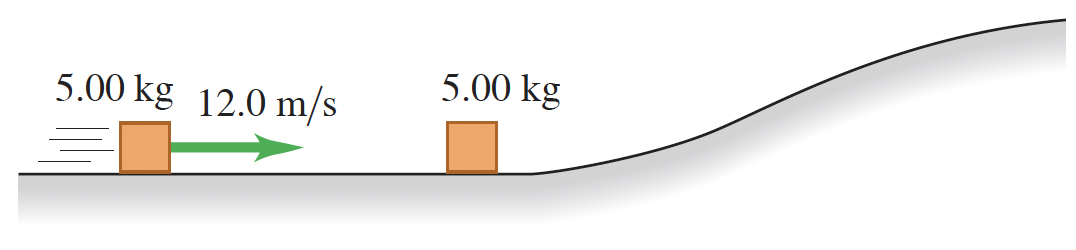
\includegraphics[width=0.5\linewidth]{../figures/P8_73.png}
  \label{fig:P8_73}
\end{figure}

A \qty{5,00}{kg} chunk of ice is sliding at \qty{12,0}{m/s} on the floor of an ice-covered valley when it collides with and sticks to another \qty{5,00}{kg} chunk of ice that is initially at rest (\textbf{\autoref{fig:P8_73}}). Since the valley is icy, there is no friction. After the collision, how high above the valley floor will the combined chunks go?
\bigbreak
I starten er den kinetiske energi givet ved
\[
k_0 = \frac{1}{2}\cdot \qty{5,00}{kg}\cdot \left( \qty{12,0}{\frac{m}{s}} \right)^2 = \qty{360}{J}
.\] 
Det antages at al denne kinetiske energi omdannes til potentiel energi som de to blokke glider op ad bakken. Altså har vi
\[
U_t = m\cdot g\cdot h \implies h = \frac{\qty{360}{J}}{\qty{10,00}{kg} \cdot \qty{9,81}{\frac{m}{s^2}}} = \qty{3,67}{m}
.\] 

\section*{Opg. 8.81}

\begin{figure} [ht]
  \centering
  \caption{}
  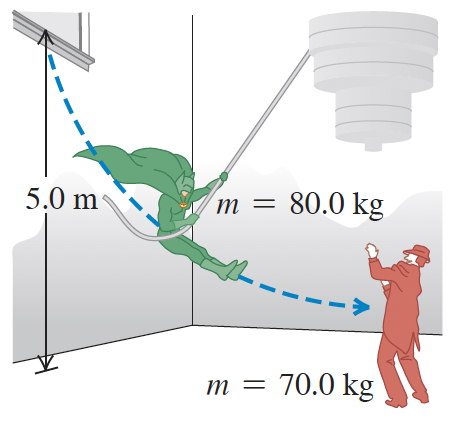
\includegraphics[width=0.5\linewidth]{../figures/P8_81.png}
  \label{fig:P8_81}
\end{figure}

A movie stuntman (mass \qty{80,0}{kg}) stands on a window ledge \qty{5,0}{m} above the floor (\textbf{\autoref{fig:P8_81}}). Grabbing a rope attached to a chandelier, he swings down to grapple with the movie’s villain (mass \qty{70,0}{kg}), who is standing directly under the chandelier. (Assume that the stuntman’s center of mass moves downward \qty{5,0}{m}. He releases the rope just as he reaches the villain.)

\subsection*{(a)}
With what speed do the entwined foes start to slide across the floor?
\bigbreak
Fra konservation af energi har vi at
\[
m_s\cdot g\cdot h = \frac{1}{2}\cdot m_s \cdot v_s^2 \implies v = \sqrt{2gh} = \sqrt{2\cdot \qty{9,81}{\frac{m}{s^2}}\cdot \qty{5,0}{m}} = \qty{9,9}{\frac{m}{s}}  
.\] 
Og fra konservation af impuls har vi at
\[
m_s\cdot v_s + 0 = (m_s + m_v)\cdot v_{sv} \implies v_{sv} = \frac{m_s\cdot v_s}{m_s+m_v} = \frac{\qty{80,0}{kg}\cdot \qty{9,9}{\frac{m}{s}}}{\qty{80,0}{kg} + \qty{70,0}{kg}} = \qty{5,28}{\frac{m}{s}} 
.\] 

\subsection*{(b)}
If the coefficient of kinetic friction of their bodies with the floor is $\mu_k = \num{0,250}$, how far do they slide?
\bigbreak
De stopper med at glide når arbejdet af fiktionskraften tilsvarer den kinetiske energi. Altså har vi
\[
\frac{1}{2}\cdot m_{sv}\cdot v_{sv}^2 = m_{sv}\cdot g\cdot \mu_k \cdot s \implies s = \frac{v_{sv}^2}{2g\cdot \mu_k} = \frac{\left( \qty{5,28}{\frac{m}{s}} \right)^2 }{2\cdot \qty{9,81}{\frac{m}{s^2}}\cdot \num{0,250}} = \qty{5,68}{m}
.\] 



\section*{Opg. 8.92}

\begin{figure} [ht]
  \centering
  \caption{}
  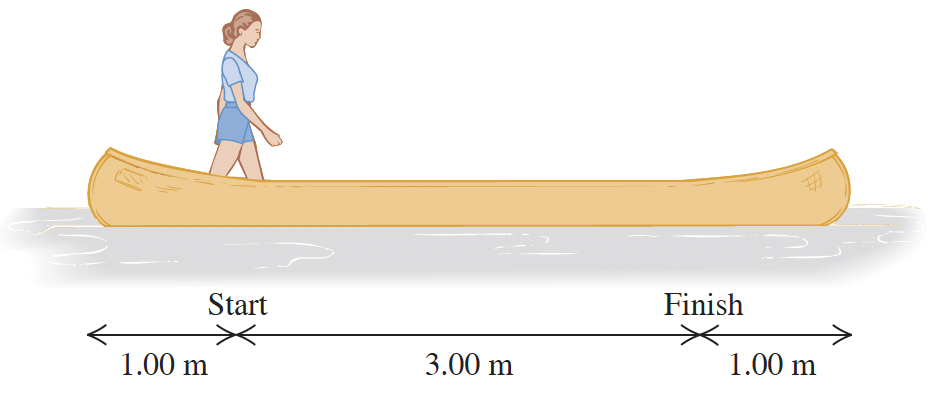
\includegraphics[width=0.5\linewidth]{../figures/P8_92.png}
  \label{fig:P8_92}
\end{figure}

A \qty{45,0}{kg} woman stands up in a \qty{60,0}{kg} canoe \qty{5,00}{m} long. She walks from a point \qty{1,00}{m} from one end to a point \qty{1,00}{m} from the other end (\textbf{\autoref{fig:P8_92}}) . If you ignore resistance to motion of the canoe in the water, how far does the canoe move during this process?
\bigbreak
Fra konservation af impuls har vi at
\[
m_w\left( v_w + v_c \right) + m_c \cdot  v_c = 0
.\] 
Vi kan dividere med tiden på begge sider af lighedstegnet
\[
m_w(x_w + x_c) + m_c \cdot x_c = 0 \implies m_w(x_w + x_c) = - m_c \cdot x_c
.\] 
Og dernæst kan vi omskrive så
\[
x_c(m_w + m_c) = - m_w x_w \implies x_c = -\frac{m_w x_w}{m_w + m_c} = -\frac{\qty{45,0}{kg}\cdot \qty{3,00}{m}}{(\qty{45,0}{kg} + \qty{60,0}{kg}} = -\qty{1,29}{m}
.\] 
Altså flytter kanoen sig \qty{1,29}{m} til venstre.

\end{document}
